\section{Пересчет динамических приоритетов}

\subsection{UNIX/LINUX}

Планирование процессов в UNIX основано на приоритете процесса.
Планировщик всегда выбирает процесс с наивысшим приоритетом. Приоритет
процесса не является фиксированным и динамически изменяется системой
в зависимости от использования вычислительных ресурсов, времени
ожидания запуска и текущего состояния процесса. Если процесс готов к
запуску и имеет наивысший приоритет, планировщик приостановит
выполнение текущего процесса (с более низким приоритетом), даже
если последний не <<выработал>> свой временной квант.

Традиционно ядро UNIX является <<непрерываемым>> (nonpreemptive).
Это означает, что процесс, находящийся в режиме ядра (в результате
системного вызова или прерывания) и выполняющий системные инструкции,
может быть прерван системой, а вычислительные ресурсы переданы другому,
более высокоприоритетному процессу. В этом состоянии выполняющийся
процесс может освободить процессор <<по собственному>> в результате
недоступности какого-либо ресурса перейдя в состояние сна. В противном
случае система может прервать выполнение процесса только при переходе
из режима ядра в режим задачи. Такой подход значительно упрощает
решение задач синхронизации и поддержания целостности структур данных
ядра.

Каждый процесс имеет два атрибута приоритета: текущий приоритет, на
основании которого происходит планирование, и заказанный
относительный приоритет, называемый nice number (или просто nice),
который задается при порождении процесса и влияет на текущий приоритет.

Текущий приоритет варьируется в диапазоне от 0 (низкий приоритет)
до 127 (наивысший приоритет). Процессы, выполняющиеся в режиме
задачи, имеют более низкий приоритет, чем в режиме ядра. Для режима
задачи приоритет меняется в диапазоне 0–65, для режима ядра --
66–95 (системный диапазон).

Процессу, ожидающему недоступного в данный момент ресурса, система
определяет значение приоритета сна выбираемое ядром из диапазона
системных приоритетов и связанное с событием, вызвавшее это состояние.

\begin{table}[H]
    \centering
    \caption{Системные приоритеты сна}
    \begin{tabular}{|l|l|l|}
        \hline
        \textbf{Событие} & \textbf{Приоритет} & \textbf{Приоритет} \\
                         & \textbf{4.3BSD UNIX} & \textbf{SCO UNIX} \\
        \hline
        \hline
        Ожидание загрузки в память сегмента/страницы & 0 & 95 \\
        (свопинг/страничное замещение) & & \\
        \hline
        Ожидание индексного дескриптора & 10 & 88 \\
        \hline
        Ожидание ввода/вывода & 20 & 81 \\
        \hline
        Ожидание буфера & 30 & 80 \\
        \hline
        Ожидание терминального ввода & & 75 \\
        \hline
        Ожидание терминального вывода & & 74 \\
        \hline
        Ожидание завершения выполнения & & 73 \\
        \hline
        Ожидание события -- низкоприоритетное состояние сна & 40 & 66 \\
        \hline
    \end{tabular}
\end{table}

В UNIX структура proc содержит следующие поля, относящиеся к приоритетам:

\begin{table}[H]
    \centering
    \begin{tabular}{|c||l|}
        \hline
        {\ttfamily p\_pri} &
        Текущий приоритет планирования \\
        \hline
        {\ttfamily p\_usrpri} &
        Приоритет режима задачи \\
        \hline
        {\ttfamily p\_cpu} &
        Результат последнего измерения использования процессора \\
        \hline
        {\ttfamily p\_nice} &
        Фактор nice, устанавливаемый пользователем \\
        \hline
    \end{tabular}
\end{table}

Когда процесс находится в режиме задачи, значение его
{\ttfamily p\_pri} идентично {\ttfamily p\_usrpri}. Когда процесс
просыпается после блокирования в системном вызове,его приоритет будет
временно повышен для того, чтобы дать ему предпочтение для выполнения
в режиме ядра. Когда заблокированный процесс просыпается, ядро
устанавливает значение его {\ttfamily p\_pri}, равное приоритету сна
события или ресурса (в диапазоне 0–49). Такой подход позволяет быстро
завершить системный вызов, выполнение которого, в свою очередь,
может блокировать некоторые системные ресурсы и приводить к
бесконечному откладыванию. Когда процесс завершил выполнение
системного вызова и находится в состоянии возврата в режим задачи,
его приоритет сбрасывается обратно в значение текущего приоритета в
режиме задачи. Это может привести к понижению приоритета, что, в
свою очередь, вызовет переключение кон- текста. На каждом тике
обработчик таймера увеличивает {\ttfamily p\_cpu} на единицу для
текущего процесса до максимального значения. Каждую секунду ядро
системы вызывает процедуру {\ttfamily schedcpu()} (запускаемую через
отложенный вызов), которая уменьшает значение {\ttfamily p\_cpu}
каждого процесса исходя из фактора <<полураспада>> (decay factor).

\begin{equation}
    \text{decay} =
    \frac
        {2 \cdot \text{load\_average}}
        {2 \cdot \text{load\_average} + 1}
\end{equation}

где load\_average — это среднее количество процессов, находящихся в состоянии готов- ности к выполнению, за последнюю секунду. Фактор полураспада обеспечивает экспонен- циально взвешенное среднее значение использования процессора в течение всего периода функционирования процесса.

Процедура schedcpu() также пересчитывает приоритеты для режима задачи всех процессов по формуле:

\begin{equation}
    \text{p\_usrpri} =
    PUSER +
    \frac{\text{p\_cpu}}{4} +
    2 \cdot \text{p\_nice}
\end{equation}

где PUSER — базовый приоритет в режиме задачи, равный 50.

Если процесс до вытеснения другим процессом использовал большое
количество процессорного времени, его {\ttfamily p\_cpu}
будет увеличен. Это приведет к росту значения {\ttfamily p\_usrpri}
и, следовательно, к понижению приоритета. Чем дольше процесс
простаивает в очереди на выполнение, тем больше фактор
полураспада уменьшает его {\ttfamily p\_cpu}, что приводит к
повышению его приоритета.

\subsection{Windows}

Ядро Windows не имеет центрального потока планирования.
Вместо этого, когда поток не может больше выполняться, он
сам вызывает планировщик, чтобы увидеть, не освободился ли в
результате его действий поток с более высоким приоритетом
планирования, который готов к выполнению. Если это так, то
происходит переключение потоков.

Поскольку Windows является полностью вытесняющей, то есть
переключение потоков может произойти в любой момент, а не только
в конце кванта текущего потока.

Windows использует 32 уровня приоритета, от 0 до 31. Эти значения
разбиваются на части следующим образом:

\begin{itemize}
    \item[--] шестнадцать уровней реального времени (от 16 до 31);
    \item[--] шестнадцать изменяющихся уровней (от 0 до 15), из
        которых уровень 0 зарезервирован для потока обнуления страниц.
\end{itemize}

\begin{figure}[H]
    \centering
    
\includegraphics[scale=0.7]{priority_levels}
    \caption{Уровни приоритета потоков}
\end{figure}

Уровни приоритета потоков назначаются исходя из двух разных позиций:
одной от Windows API и другой от ядра Windows. Сначала Windows API
систематизирует процессы по классу приоритета, который им присваивается
при создании: Реального времени -- Real-time (4), Высокий -- High (3),
Выше обычного — Above Normal (7), Обычный -- Normal (2), Ниже
обычного -- Below Normal (5) и Простоя -- Idle (1).

Затем назначается относительный приоритет отдельных потоков внутри
этих процессов. Здесь номера представляют изменение приоритета,
применяющееся к базовому приоритету процесса: Критичный по времени
-- Time-critical (15), Наивысший -- Highest (2), Выше обычного --
Above-normal (1), Обычный -- Normal (0), Ниже обычного -- Below-normal
(–1), Самый низший -- Lowest (–2) и Простоя -- Idle (–15).

Поэтому в Windows API каждый поток имеет базовый приоритет,
являющийся функцией класса приоритета процесса и его относительног
приоритета процесса. В ядре класс приоритета процесса преобразуется
в базовый приоритет путем ис- пользования процедуры PspPriorityTable
и показанных ранее индексов PROCESS\_PRIORITY\_CLASS, устанавливающих
приоритеты 4, 8, 13, 14, 6 и 10 соответственно. (Это фиксированное
отображение, которое не может быть изменено.) Затем при- меняется
относительный приоритет потока в качестве разницы для этого базового
приоритета. Например, наивысший «Highest»-поток получит базовый
приоритет потока на два уровня выше, чем базовый приоритет его процесса.

\begin{table}[H]
    \centering
    \caption{Отображение приоритетов ядра Windows на Windows API}
    \begin{tabular}{|l|l|l|l|l|l|l|}
        \hline
        \textbf{Класс приоритета/} &
        \textbf{Realtime} &
        \textbf{High} &
        \textbf{Above} &
        \textbf{Normal} &
        \textbf{Below} &
        \textbf{Idle} \\
        \textbf{Относительный приоритет} & & &
        \textbf{Normal} & & \textbf{Normal} & \\
        \hline
        \hline
        Time Critical (+ насыщение) & 31 & 15 & 15 & 15 & 15 & 15 \\
        \hline
        Highest (+2) & 26 & 15 & 12 & 10 & 8 & 6 \\
        \hline
        Above Normal (+1) & 25 & 14 & 11 & 9 & 7 & 5 \\
        \hline
        Normal (0) & 24 & 13 & 10 & 8 & 6 & 4 \\
        \hline
        Below Normal (--1) & 23 & 12 & 9 & 7 & 5 & 3 \\
        \hline
        Lowest (--2) & 22 & 11 & 8 & 6 & 4 & 2 \\
        \hline
        Idle (-- насыщение) & 16 & 1 & 1 & 1 &1 & 1 \\
        \hline
    \end{tabular}
\end{table}

Для использования этих приоритетов при планировании система
поддерживает массив из 32 списков потоков, соответствующих всем
32 приоритетам (от 0 до 31). Каждый список содержит готовые потоки
соответствующего приоритета. Базовый алгоритм планирования делает
поиск по массиву от приоритета 31 до приоритета 0. Как только будет
найден непустой список, поток выбирается сверху списка и выполняется
в течение одного кванта. Если квант истекает, то поток переводится в
конец очереди своего уровня приоритета и следующим выбирается верхний
поток списка. Если готвых потоков нет, то процессор переходит в
состояние ожидания, то есть переводится в состояние более низкого
энергопотребления и ждет прерывания.

Потоки приложений обычно выполняются с приоритетами 1–15.
Как правило, пользовательские приложения и службы запускаются
с обычным базовым приоритетом (normal), поэтому их исходный
поток чаще всего выполняется с уровнем приоритета 8.

Повышение приоритета вступает в действие немедленно и может
вызвать изменения в планировании процессора. Однако если поток
использует весь свой следующий квант, то он теряет один уровень
приоритета и перемещается вниз на одну очередь в массиве приоритетов.
Если же он использует второй полный квант, то он перемещается вниз
еще на один уровень, и так до тех пор, пока не дойдет до своего
базового уровня (где и останется до следующего повышения).

Повышение приоритета потока в Windows применяется только для потоков
с приоритетом динамического диапазона ( 0-15). Но каким бы ни было
приращение, приоритет потока никогда не будет больше 15. Таким образом,
если к потоку с приоритетом 14 применить динамическое повышение на 5
у ровней, т о его приоритет станет равным только 15 (если приоритет
потока равен 15, то повысить его нельзя).

\begin{table}[H]
    \centering
    \caption{Рекомендуемые значения повышения приоритета}
    \begin{tabular}{|l|l|}
        \hline
        \textbf{Устройство} & \textbf{Повышение приоритета} \\
        \hline
        \hline
        Жесткий диск, привод компакт-дисков & 1 \\
        параллельный порт, видеоустройство & \\
        \hline
        Сеть, почтовый слот, именованный канал, & 2 \\
        последовательный порт & \\
        \hline
        Клавиатура, мышь & 6 \\
        \hline
        Звуковое устройство & 8 \\
        \hline
    \end{tabular}
\end{table}

Приоритет потока повышается:

\begin{itemize}
    \item[--] Когда операция ввода-вывода завершается и освобождает
        находящийся в состоянии ожидания поток, то его приоритет
        повышается (чтобы он мог опять быстро запуститься и начать
        новую операцию ввода-вывода). Важно, что для запросов на
        ввод/вывод, адресованных у стройством с меньшим гарантированным
        временем отклика, предусматриваются большие приращения
        приоритета.
    \item[--] Если поток ждал на семафоре, мьютексе или другом событии,
        то при его освобождении он получает повышение приоритета на
        два уровня, если находится в фоновом процессе, и на один
        уровень во всех остальных случаях. Это целесообразно, так
        как потокам, блокируемым на событиях, процессорное время
        требуется реже, чем остальным (это позволяет равномернее
        распределять процессорное время).
    \item[--]  Если поток графического интерфейса пользователя
        просыпается по причине наличия ввода от пользователя,
        то он также получает повышение.
    \item[--]  Если поток, готовый к выполнению, задерживается из-за
        нехватки процессорного времени. Раз в секунду диспетчер
        настройки баланса (системный поток, предназначенный главным
        образом для выполнения функций управления памятью), проверяет
        очереди готовых потоков и ищет потоки, которые находятся в
        состоянии готовности (Ready) в течение 4 секунд. Обнаружив
        такой поток, диспетчер настройки баланса повышает его приоритет
        до 15. В Windows 2000 и Windows ХР квант потока удваивается
        относительно кванта процесса. В Windows Server 2003 квант
        устанавливается равным 4 единицам. Как только квант истекает,
        приоритет потока немедленно снижается до исходного уровня.
        Если этот поток не успел закончить свою работу и если другой
        поток с более высоким приоритетом готов к выполнению, то после
        снижения приоритета он возвращается в очередь готовых потоков.
        В итоге через 4 секунды его приоритет может быть снова
        повышен. Чтобы свести к минимуму расход процессорного времени,
        диспетчер настройки баланса сканирует лишь 16 готовых потоков.
        Если таких потоков с данным уровнем приоритета более 16, он
        запоминает тот поток, перед которым он остановился, и в
        следующий раз продолжает сканирование именно с него. Кроме
        того, он повышает приоритет не более чем у 10 потоков за
        один проход. Обнаружив 10 потоков, приоритет которых следует
        повысить (что говорит о высокой загруженности системы), он
        прекращает сканирование. При следующем проходе сканирование
        возобновляется с того места, где оно было прервано в
        прошлый раз.
\end{itemize}

Для обеспечения поддержки мультизадачности системы, когда
исполняется код режима ядра, Windows использует приоритеты
прерываний IRQL.

\begin{figure}[H]
    \centering
    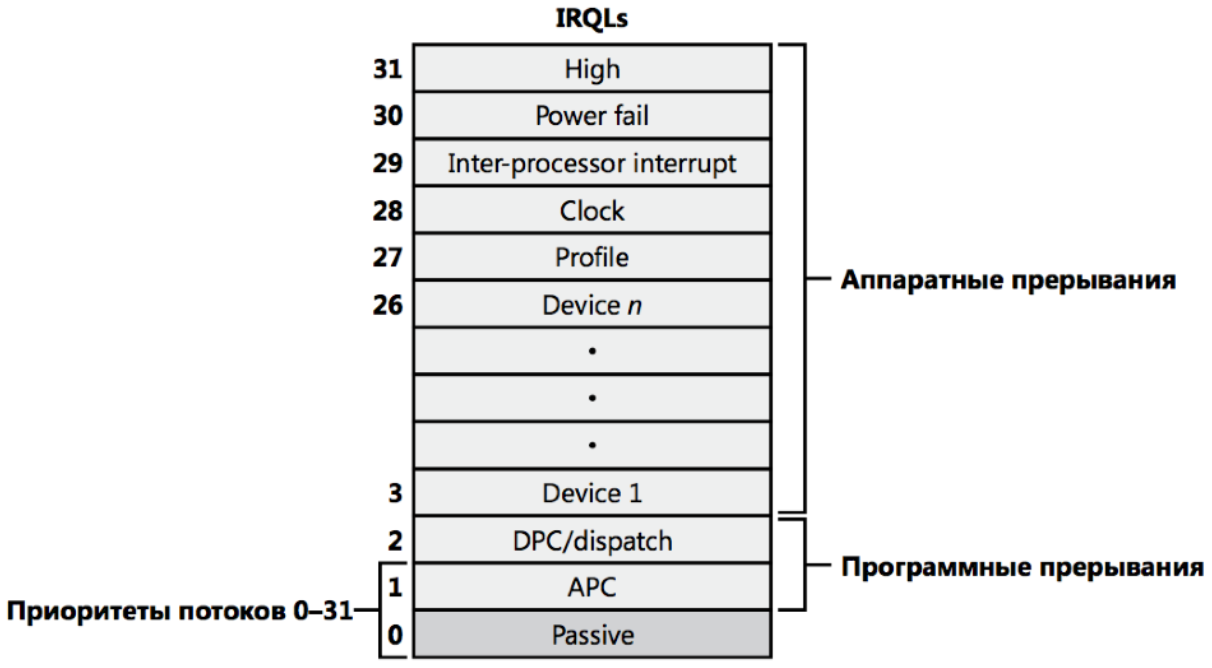
\includegraphics[scale=0.8]{irql}
    \caption{Сопоставление приоритетов потоков с IRQL-уровнями}
\end{figure}

Потоки, запущенные в режиме ядра, несмотря на изначальное планирование
на пассивном уровне или уровне APC, могут поднять IRQL на более
высокие уровни.

Если поток поднимает IRQL на уровень dispatch или еще выше, на
его процессоре не будет больше происходить ничего, относящегося
к планированию потоков, пока уровень IRQL не будет опущен ниже
уровня dispatch. Поток выполняется на dispatch-уровне и выше,
блокирует активность планировщика потоков и мешает контекстному
переключению на своем процессоре.

Поток, запущенный в режиме ядра, может быть запущен на APC-уровне,
если он запускает специальный APC-вызов ядра, или он может временно
поднять IRQL до APC-уровня, чтобы заблокировать доставку специальных
APC-вызовов ядра. Поток, выполняемый в режиме ядра на APC-уровне,
может быть прерван в пользу потока с более высоким приоритетом,
запущенным в пользовательском режиме на уровне passive.
